\section{Experimental approach}
\label{sec:experimental_approach}

As shown from a theoretical point of view in Section \ref{sec:analysis_shunted_piezo}, it's possible to control the band-gaps of a beam by means of shunted piezoelectric patches.
Experimental validation has also been performed in this sense and is presented in this section.

At first, the experimental setup is described, highlighting the configuration used for the piezoelectric patches and the shunt circuits.
Then, the experimental data are presented together with the theoretical predictions obtained through the numerical methods presented in Section \ref{subsec:numerical_methods_for_wave_propagation_analysis}.

At first, the space-only modulation is considered, and the tools used for the analysis are the Transfer Matrix Method (TMM) and the Plane Wave Expansion Method (PWEM).
\texttt{Comsol Multiphysics} is also adoperated to validate both the numerical methods results and the experimental data.
Then, the space-time modulation is considered, and the nonreciprocal behavior is highlighted showing that the experimental results are in agreement with the theoretical predictions obtained from PWEM.

\subsection{Setup}
\label{subsec:experimental_setup}

As already anticipated, material property modulation is achieved by means of shunted piezoelectric patches.
Figure \ref{fig:experimental_setup} illustrates the experimental setup, highlighting the placement of the piezoelectric patches and the shunt circuits.

\begin{figure}[H]
    \centering
    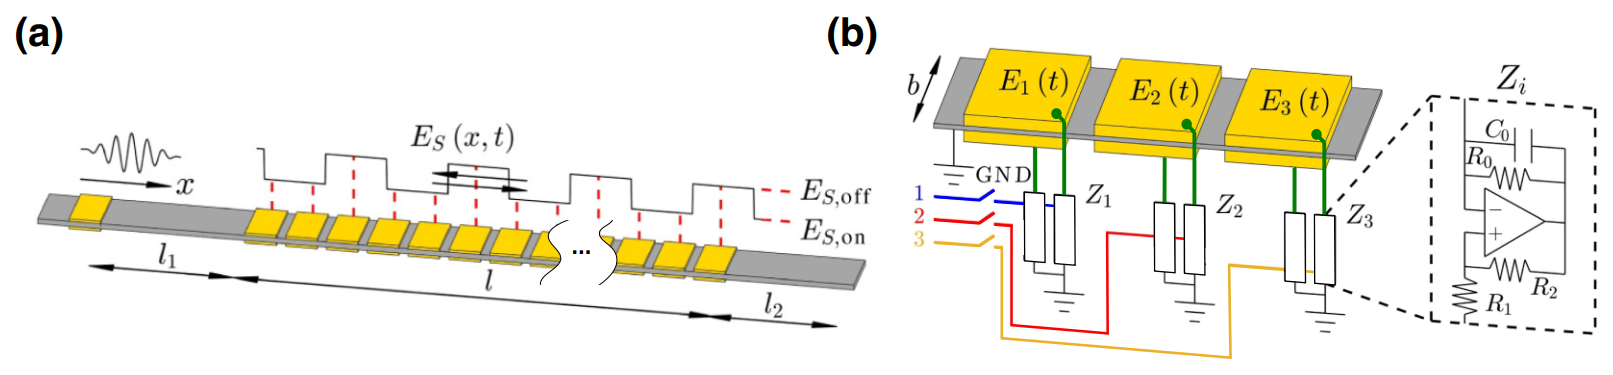
\includegraphics[width=0.9\textwidth]{./img/experimental_setup_scheme.png}
    \caption{Schematic of the experimental setup.}
    \label{fig:experimental_setup}
\end{figure}

In particular, Figure \ref{fig:experimental_setup} (a) depicts the electromechanical beam, including the excitation patch (responsible for generating the travelling wave signal) and the active domain containing the array of piezoelectric patches.
Figure \ref{fig:experimental_setup} (b) provides a close-up view of the unit spatiotemporal (ST) cell, consisting of three piezoelectric patches and the corresponding $C_N$ type shunt circuits.
Active modualtion is achieved by toggling switches that control the connection between the power supply and operational amplifiers.

The host beam consists of an aluminum substrate with a cross-section of $20 mm \times 1 mm$ and a total length of $2400 mm$.
An array of piezoelectric patches, spaced $2 mm$ apart, is positioned at $l_1 = 690 mm$ and $l_2 = 1134 mm$ from the beam's left and right boundaries, respectively.
This choice of placement minimizes boundary reflections, further mitigated by the use of absorbing boundary layers composed of mastic tape.

The active piezoelectric region, spanning $576 mm$, consists of $24$ pairs of piezoelectric patches with dimensions $20 mm \times 22 mm \times 1 mm$.
These patches are bonded on opposite surfaces of the beam and connected to a total of $48$ negative capacitance shunt circuits.
When the circuit is closed, the effective stiffness of the beam section is reduced (see Equation \ref{eq:weighted_average_mechanical_properties}).

The out-of-plane velocity field along the beam's length is measured using a Polytec 3D laser Doppler vibrometer (SLDV).

In Table \ref{tab:experimental_setup_parameters}, the main parameters of the experimental setup are summarized.

\begin{table}[H]

    \centering

    \begin{tabular}{|l|c|c|c|}
        \hline
        \textbf{Parameter}                 & \textbf{Symbol} & \textbf{Value} & \textbf{Units} \\
        \hline
        Beam Young's modulus               & $Y_b$           & $69$           & $GPa$          \\
        Beam density                       & $\rho_b$        & $2700$         & $kg/m^3$       \\
        \hline
        Piezoelectric Young's modulus      & $Y_1^E$         & $62$           & $GPa$          \\
        Piezoelectric capacitance          & $C_T$           & $7.0$          & $nF$           \\
        Piezoelectric coupling coefficient & $k_{31}$        & $0.351$        & -              \\
        Piezoelectric density              & $\rho$          & $7900$         & $kg/m^3$       \\
        \hline
        Shunt capacitance                  & $C_0$           & $4.4$          & $nF$           \\
        Shunt bias resistance              & $R_0$           & $1.0$          & $M\Omega$      \\
        Shunt resistance                   & $R_1$           & $7.5$          & $k\Omega$      \\
        Shunt resistance                   & $R_2$           & $13.7$         & $k\Omega$      \\
        \hline
    \end{tabular}

    \caption{Main parameters of the experimental setup.}
    \label{tab:experimental_setup_parameters}

\end{table}
\subsection{Space-Only Modulation}
\label{subsec:space_only_modulation}

In the case of space-only modulation, a given pair of piezoelectric patches can be either in the short-circuit or open-circuit state.
For simplicity, we will refer to these states as ON and OFF, respectively.

Considering the ST cell as composed by three pairs of piezoelectric patches, three different configurations are analyzed:

\begin{itemize}
    \item OFF-OFF-OFF: all the shunt circuits are open;
    \item ON-ON-ON: all the shunt circuits are closed;
    \item OFF-OFF-ON: only the last shunt circuit is closed.
\end{itemize}

The mechanical properties of the system are computed so to obtain $EJ(x)$ and $\rho A(x)$, which are then used by the numerical methods to compute the dispersion diagram of the system.
In the following, the results of the numerical simulations are compared with the experimental data.

Both the TMM and PWEM are expected to exhibit some discrepancies with the experimental data at higher frequencies due to the hypothesis made in the theoretical model.
The Euler-Bernoulli beam theory that has been used in the theoretical model, is known to be a good approximation only for low-frequency excitations and small deformations.
Timošenko beam theory could have been a better choice, but it would have made the theoretical model more complex and the numerical simulations more computationally expensive.

Moreover, for the PWEM, a number of space and time harmonics equal to $P = 40$ and $Q = 1$ are considered, respectively.
The relative low number of space harmonics is expected to introduce some additional discrepancies with the experimental data, especially at higher frequencies.

\texttt{Comsol Multiphysics} is used as a valid reference to validate the experimental results given that internal losses and higher order modes are taken into account into its numerical solvers.


\paragraph{OFF-OFF-OFF}

The first case considered is the OFF-OFF-OFF configuration, where all the shunt circuits are open.
In this case, based on Equation \ref{eq:mechanical_admittance_shunted_piezoelectric_patch}, the piezo's mechanical admittance is given by:

\begin{equation}
    Y^{SU} = Y_1^D
\end{equation}

Figure \ref{fig:space_only_off_off_off}, shows the PWEM and experimental results, while the comparison between the TMM and Comsol Multiphysics is shown in Figure \ref{fig:space_only_off_off_off_comsol}.

\begin{figure}[H]
    \centering
    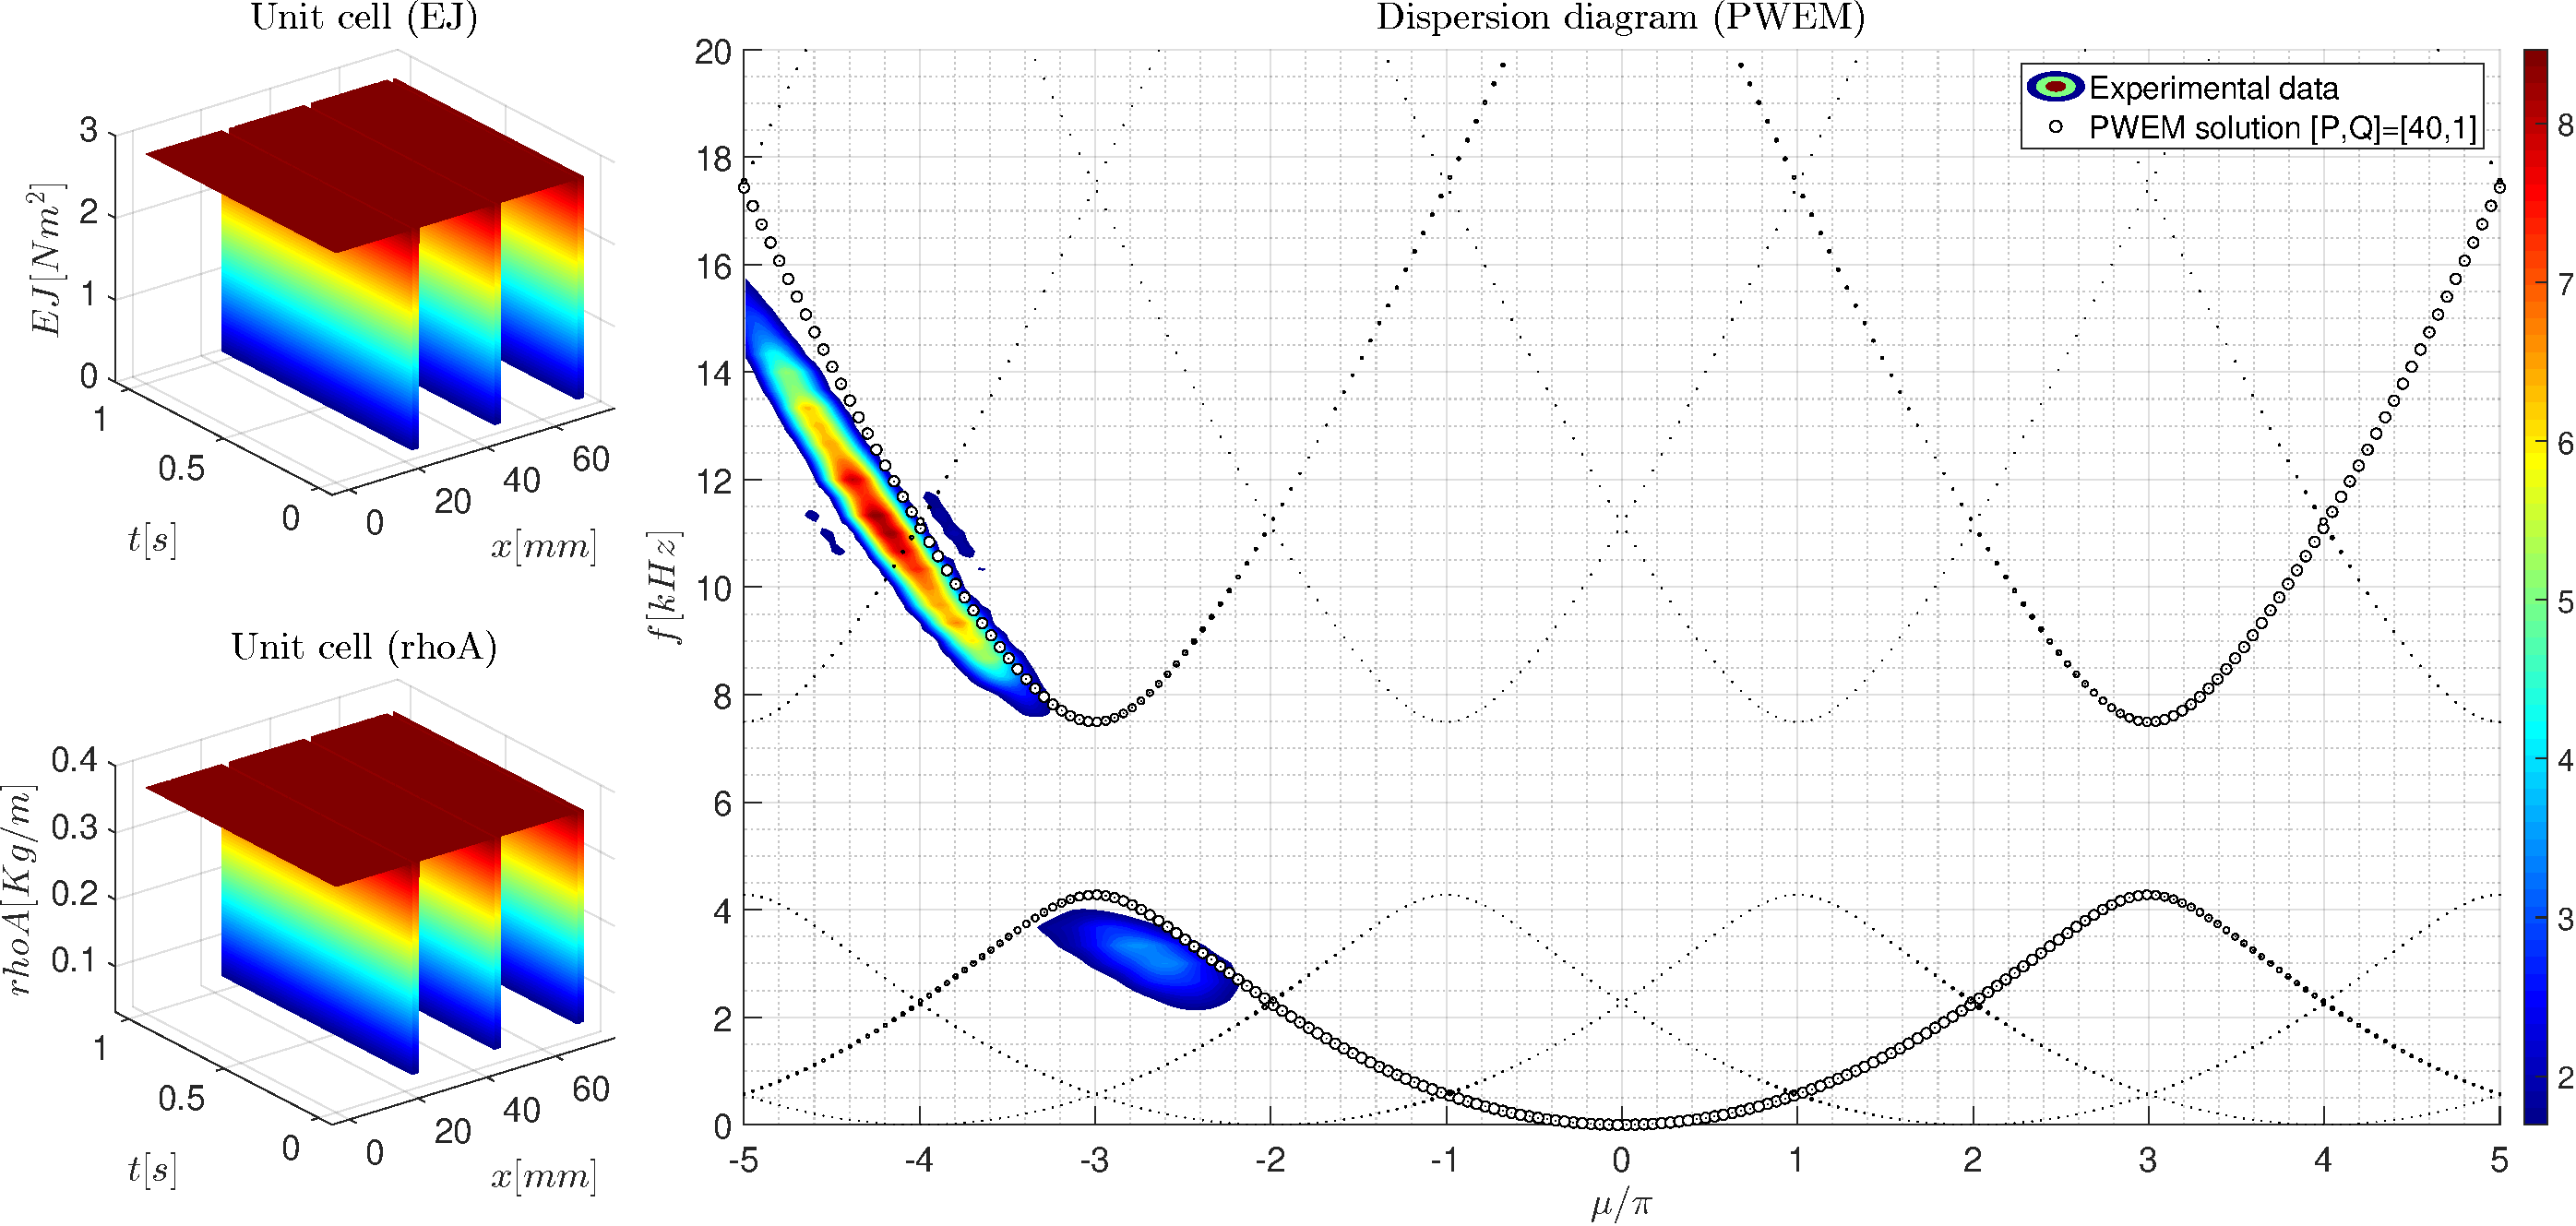
\includegraphics[width=\textwidth]{./img/MATLAB/PWEM_EXP OFF-OFF-OFF @0kHz.pdf}
    \caption{Band structure for the OFF-OFF-OFF configuration.}
    \label{fig:space_only_off_off_off}
\end{figure}

\begin{figure}[H]
    \centering
    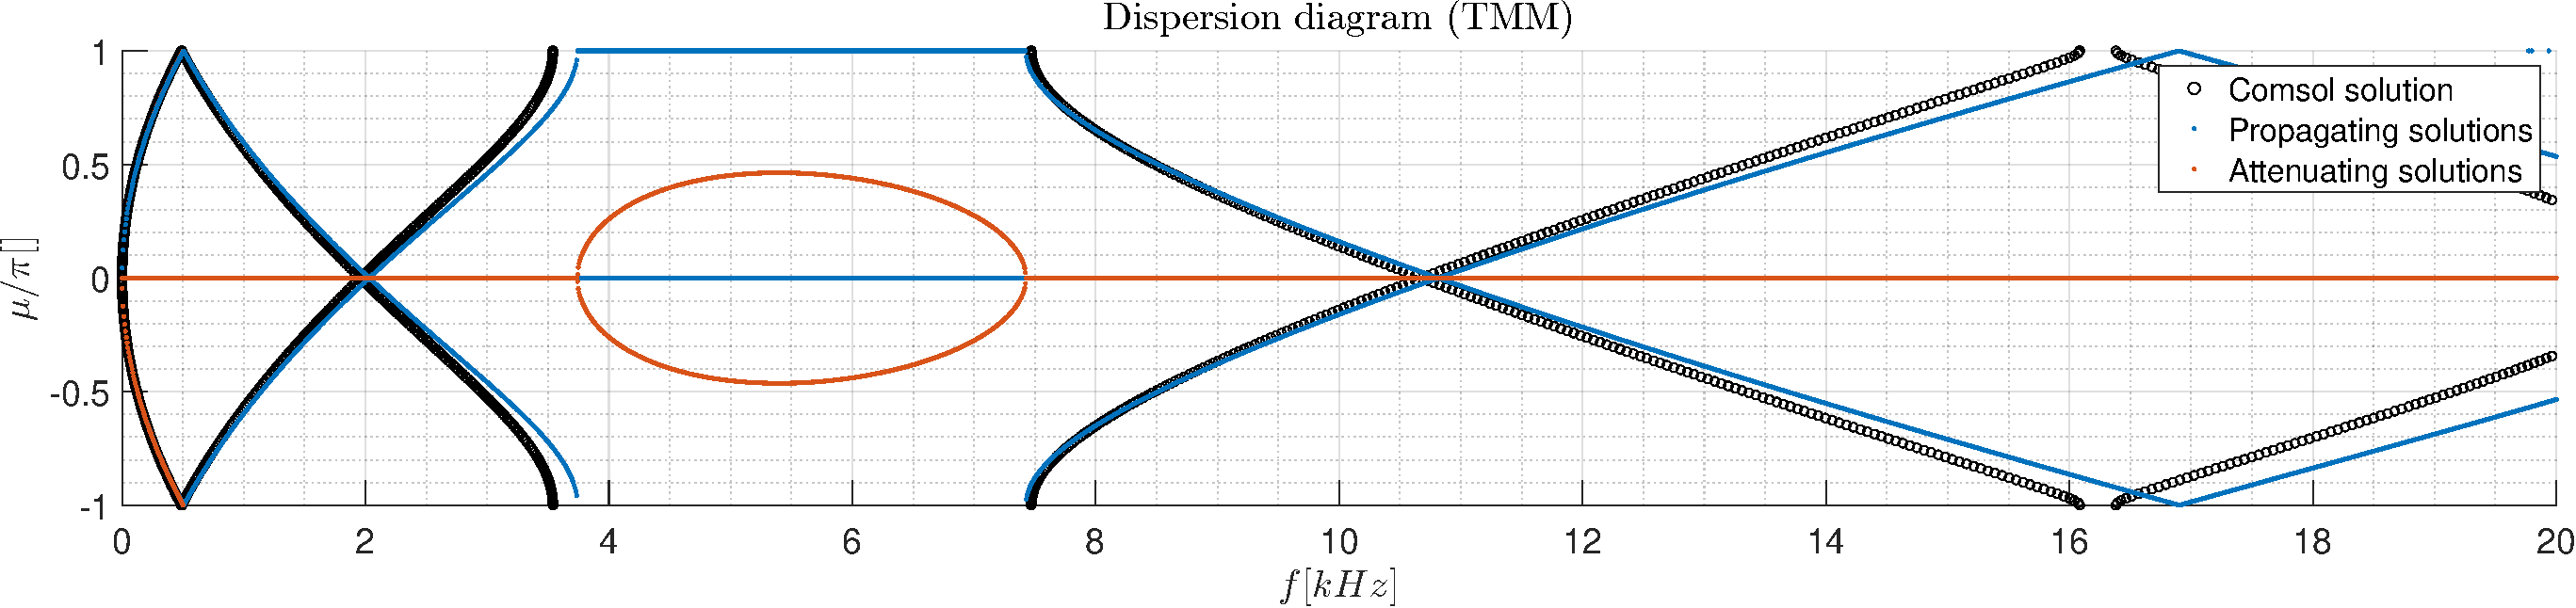
\includegraphics[width=\textwidth]{./img/MATLAB/TMM_COMSOL OFF-OFF-OFF @0kHz.pdf}
    \caption{Comparison between TMM and Comsol Multiphysics for the OFF-OFF-OFF configuration.}
    \label{fig:space_only_off_off_off_comsol}
\end{figure}

In the above figures, what has been suggested with the introductory considerations is confirmed.
Both the TMM and PWEM exhibit some discrepancies with the experimental data at higher frequencies.
However, their results are still in good agreement with the experimental data, being able to predict the band-gap position.

From the comparison between the TMM and Comsol Multiphysics, it can be seen that the TMM method underestimate the stiffness of the beam at higher frequencies, causing an upper shift of the dispersion diagram with respect to both the experimental data and the Comsol Multiphysics results.
Under the hypothesis that this offset is due to the Euler-Bernoulli assumption, we can state that the model can be considered valid for the analysis of the system.

In the case of the OFF-OFF-OFF configuration, the band gap of the structure is found at:

\begin{equation}
    f_{BG}^{OFF-OFF-OFF} = [3.8, 7.5] kHz
\end{equation}



\paragraph{ON-ON-ON}

The second case considered is the ON-ON-ON configuration, where all the shunt circuits are in the short-circuit state.
In this case, the piezo's mechanical admittance is given by:

\begin{equation}
    Y^{SU} = Y_1^E
\end{equation}

Figure \ref{fig:space_only_on_on_on}, shows the PWEM and experimental results, while the comparison between the TMM and Comsol Multiphysics is shown in Figure \ref{fig:space_only_on_on_on_comsol}.

\begin{figure}[H]
    \centering
    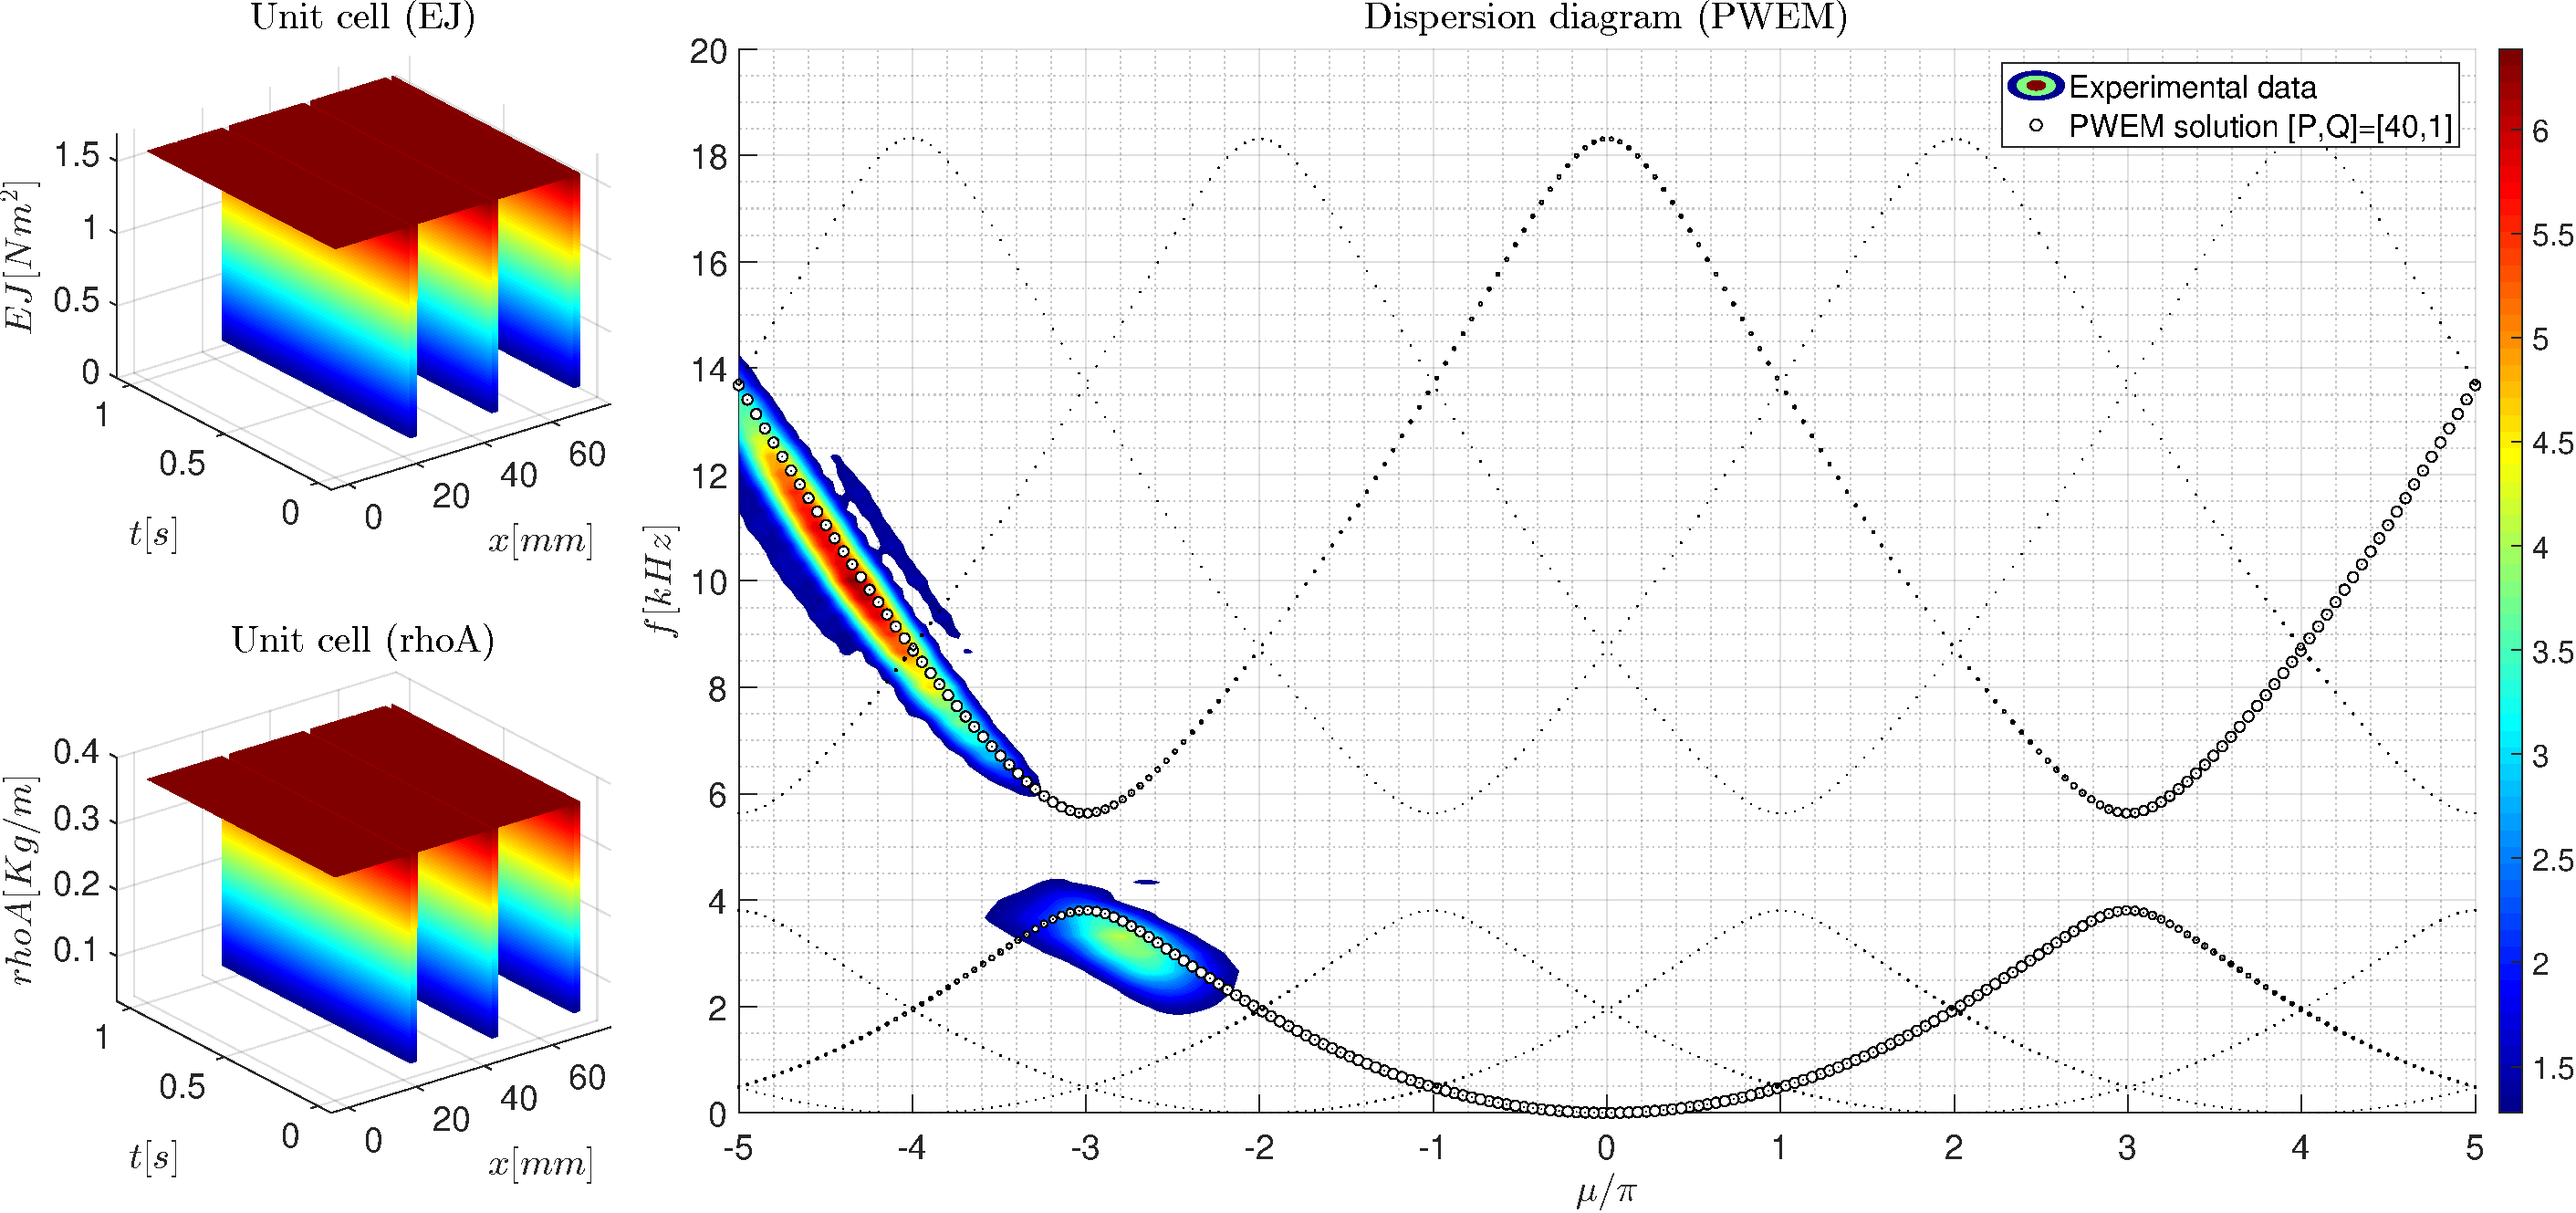
\includegraphics[width=\textwidth]{./img/MATLAB/PWEM_EXP ON-ON-ON @0kHz.pdf}
    \caption{Band structure for the ON-ON-ON configuration.}
    \label{fig:space_only_on_on_on}
\end{figure}

\begin{figure}[H]
    \centering
    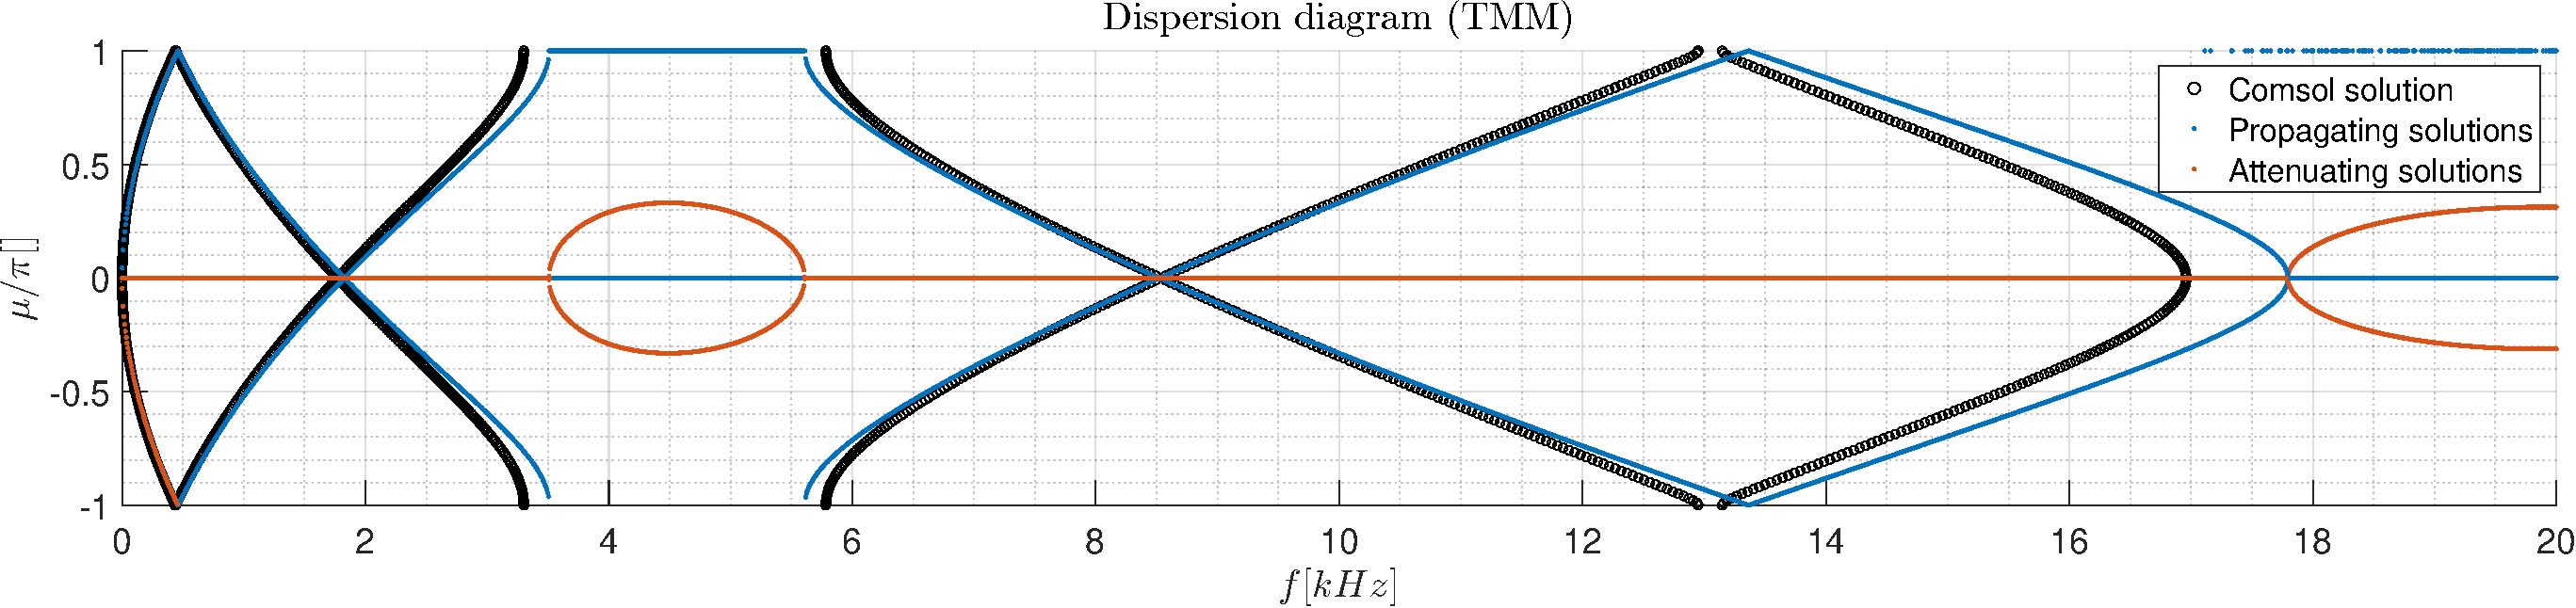
\includegraphics[width=\textwidth]{./img/MATLAB/TMM_COMSOL ON-ON-ON @0kHz.pdf}
    \caption{Comparison between TMM and Comsol Multiphysics for the ON-ON-ON configuration.}
    \label{fig:space_only_on_on_on_comsol}
\end{figure}

Similar consideration as before can be done about the discrepancy between the numerical methods and the experimental data.
Comsol Multiphysics is again used as a reference to validate the experimental results.

With respect to the ON-ON-ON configuration, a shift of the band-gap towards lower frequencies is observed:

\begin{equation}
    f_{BG}^{ON-ON-ON} = [3.4, 5.6] kHz
\end{equation}

This shift is due to the fact that the piezoelectric patches are in the short-circuit state, which results in a lower effective stiffness of the beam section.
Having a lower effective stiffness is equivalent to state that the speed of the travelling wave is lower, which results in a lower frequency of the band-gap.



\paragraph{ON-OFF-OFF}

The last case considered regarding the space-only modulation is the ON-OFF-OFF configuration, where only the first shunt circuit is closed and the other two are open.

It's intuitive to understand that the mechanical admittance is no more the same for the three piezoelectric patches.
This will introduce additional sources of dispersion in the system, which will result in higher number of band-gaps visible in the same frequency range.

Figure \ref{fig:space_only_on_off_off}, shows the PWEM and experimental results, while the comparison between the TMM and Comsol Multiphysics is shown in Figure \ref{fig:space_only_on_off_off_comsol}.

\begin{figure}[H]
    \centering
    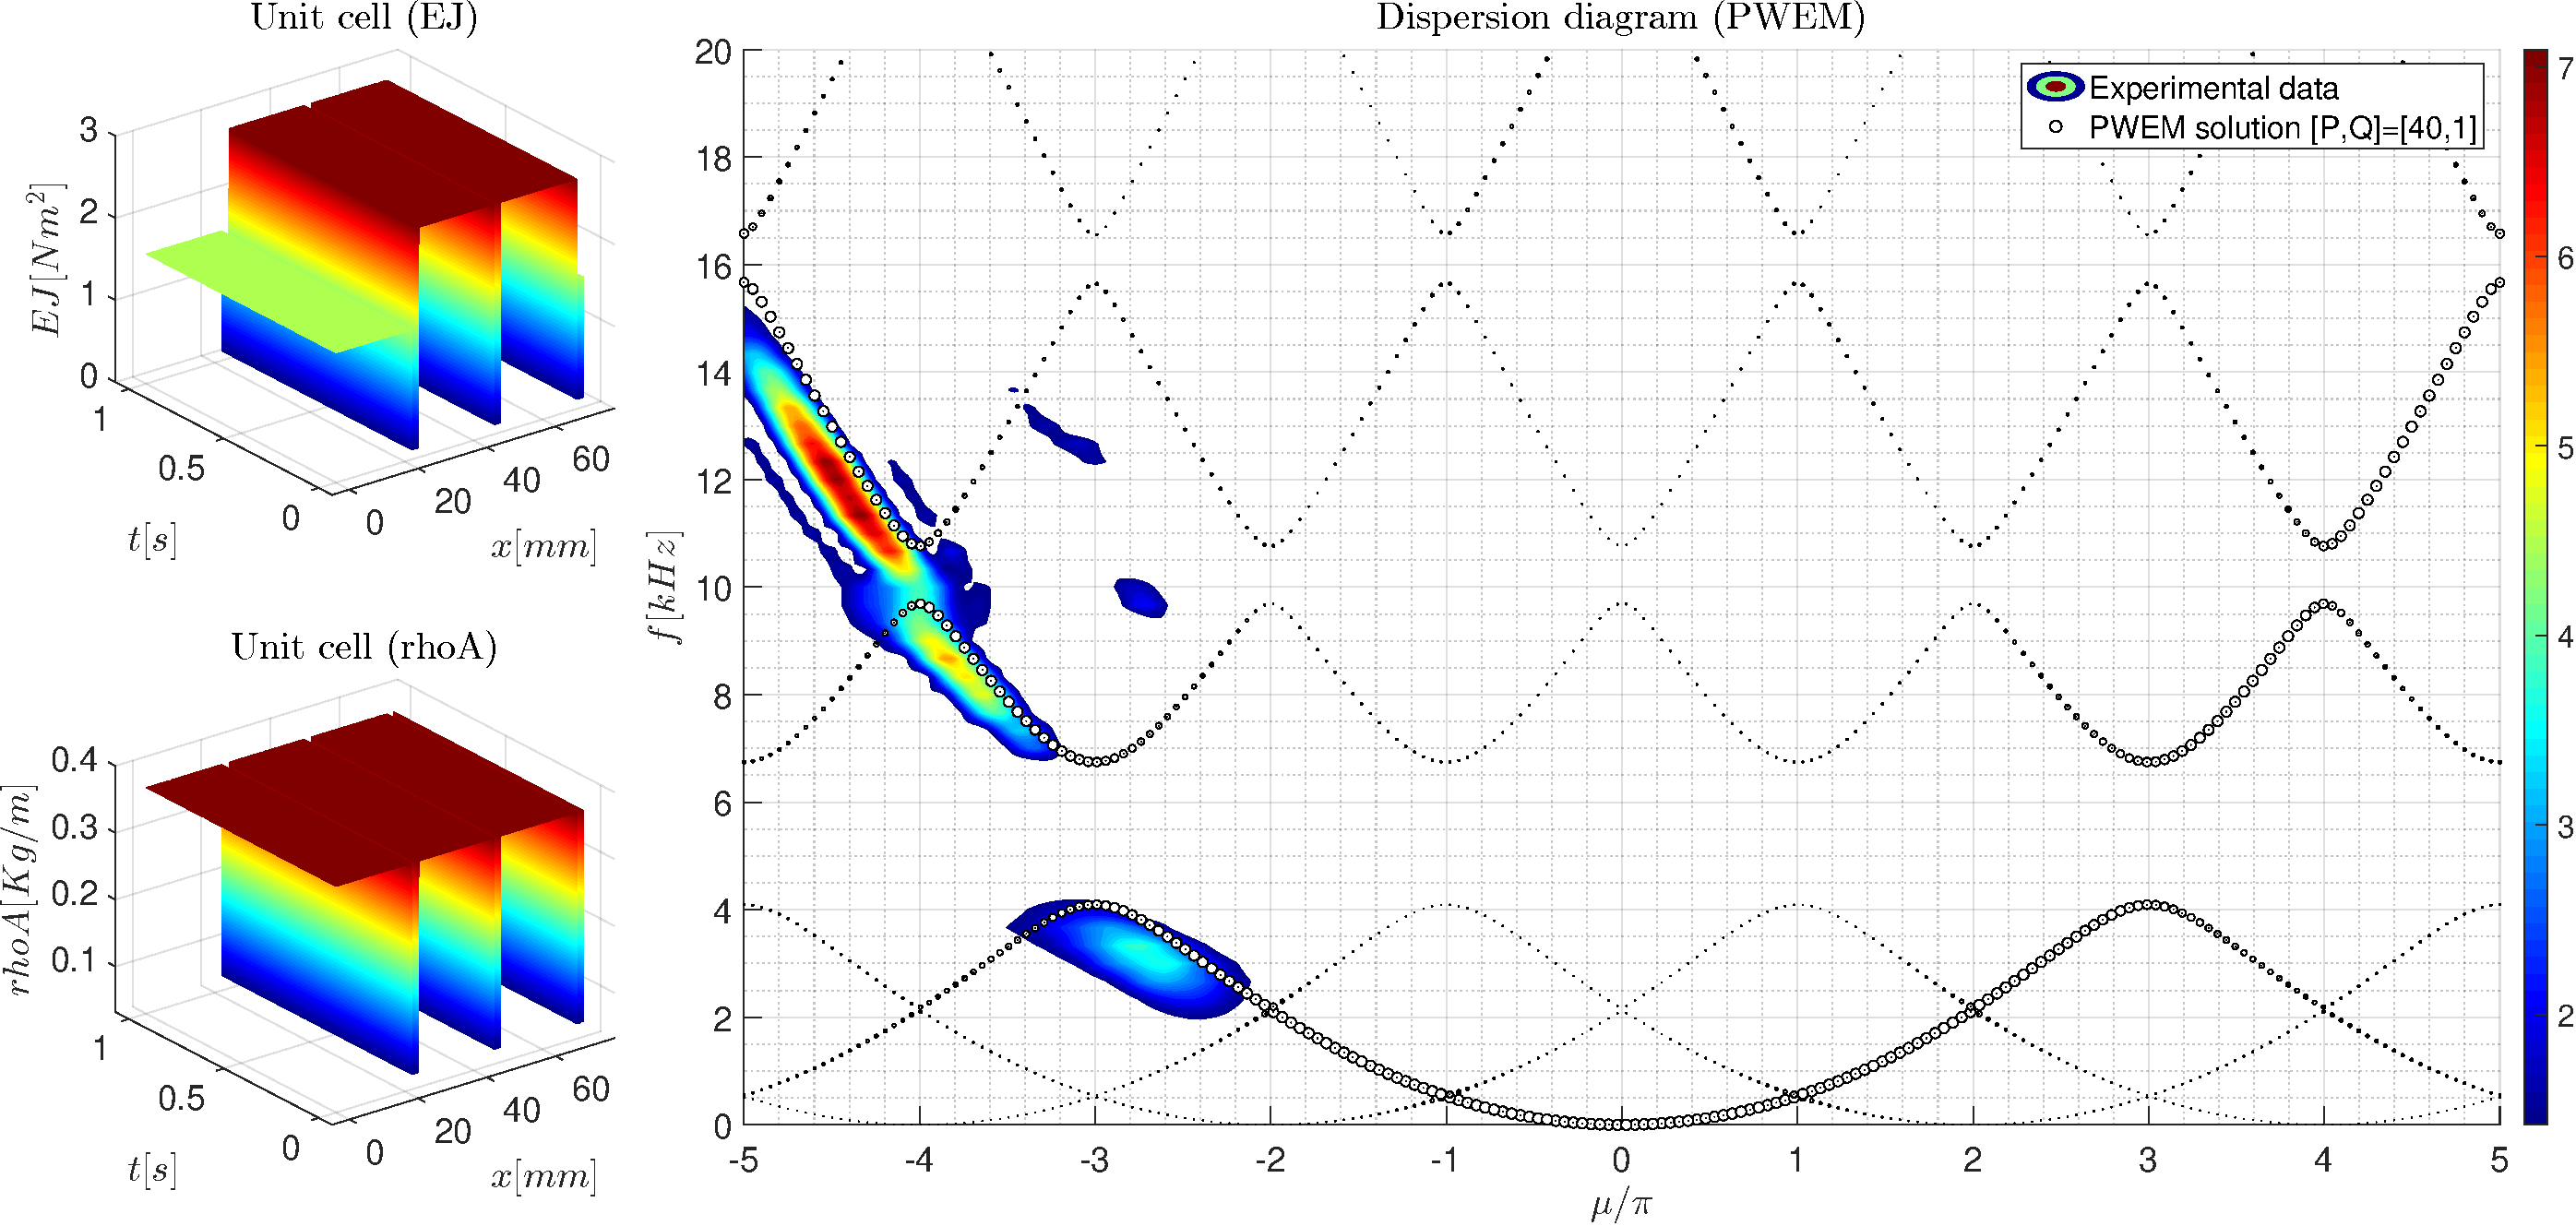
\includegraphics[width=\textwidth]{./img/MATLAB/PWEM_EXP ON-OFF-OFF @0kHz.pdf}
    \caption{Band structure for the ON-OFF-OFF configuration.}
    \label{fig:space_only_on_off_off}
\end{figure}

\begin{figure}[H]
    \centering
    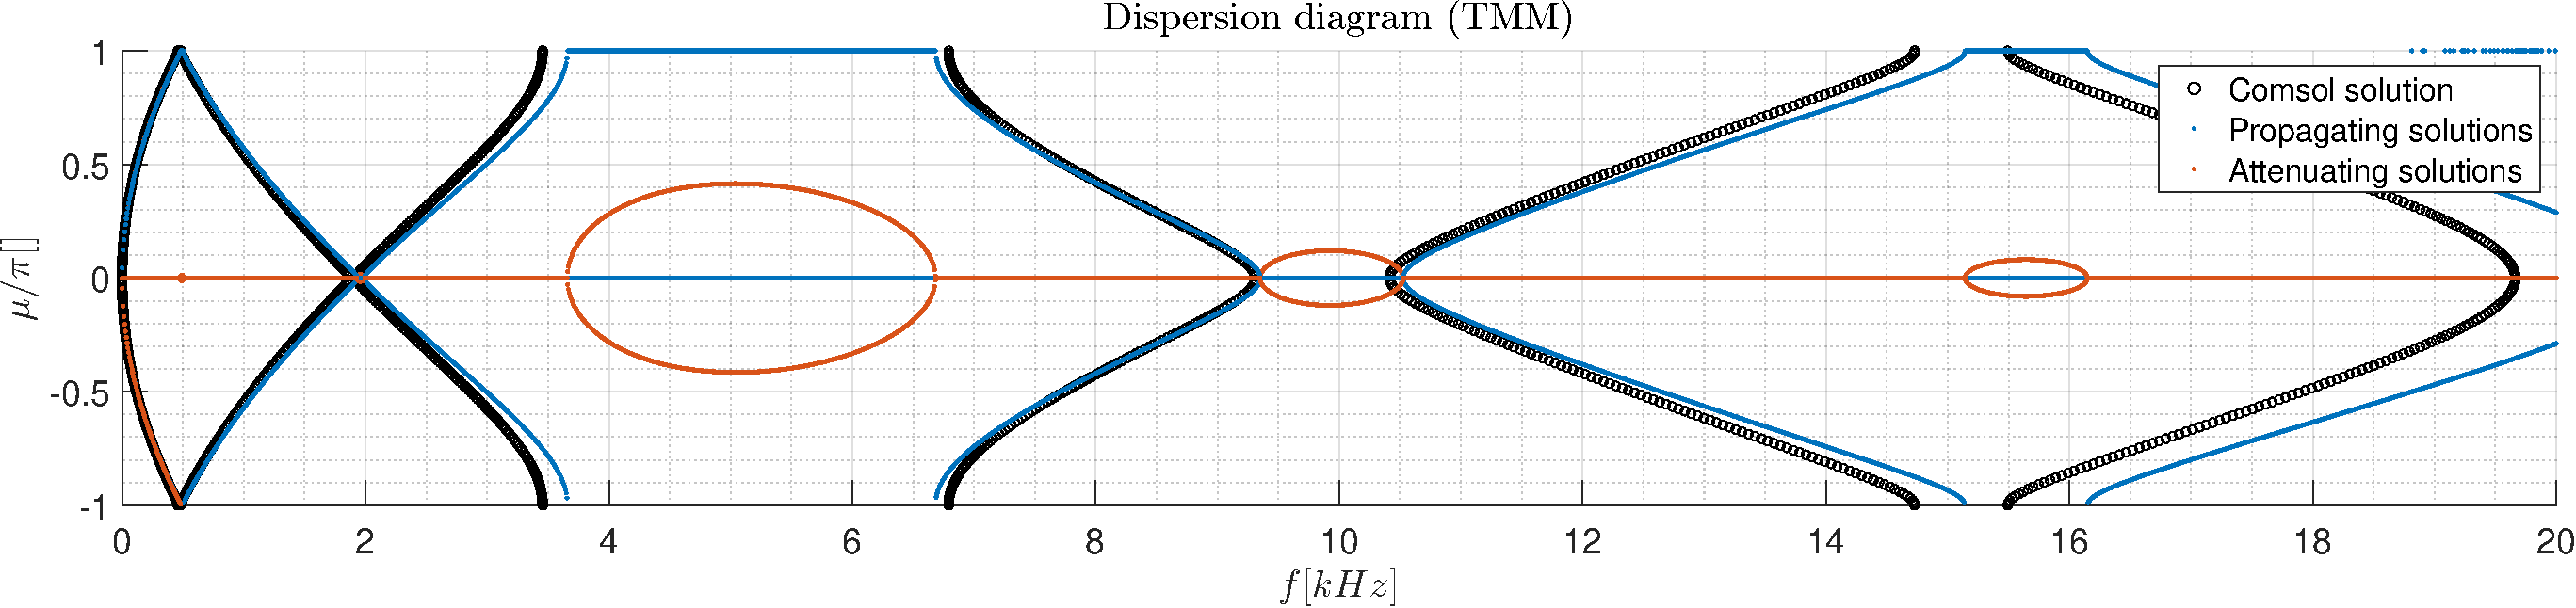
\includegraphics[width=\textwidth]{./img/MATLAB/TMM_COMSOL ON-OFF-OFF @0kHz.pdf}
    \caption{Comparison between TMM and Comsol Multiphysics for the ON-OFF-OFF configuration.}
    \label{fig:space_only_on_off_off_comsol}
\end{figure}

As a confirmation of the previous considerations, the band structure of the ON-OFF-OFF configuration shows a higher number of band-gaps in the same frequency range.

The band gap of the structure are now found at:

\begin{equation}
    \begin{aligned}
        f_{BG1}^{ON-OFF-OFF} & = [3.5, 6.7] kHz   \\
        f_{BG2}^{ON-OFF-OFF} & = [9.3, 10.4] kHz  \\
        f_{BG3}^{ON-OFF-OFF} & = [14.7, 15.5] kHz
    \end{aligned}
\end{equation}

\subsection{Space-Time Modulation}
\label{subsec:space_time_modulation}

For the case of space-time modulations, the three pairs of piezoelectric patches are driven by three equal but shifted in time signals.

The general law guiding the modulation is the following:

\begin{equation}
    Y_k^{SU} = \frac{(Y_1^D + Y_1^E)}{2} + \frac{(Y_1^D - Y_1^E)}{2} sign \left[ \cos \left( 2 \pi f_m t + (k-1) \frac{2\pi}{3} \right) \right]
\end{equation}

Where $Y_k^{SU}$ is the mechanical admittance of the $k$-th piezoelectric patch in the spatiotemporal (ST) cell, $Y_1^D$ and $Y_1^E$ are the mechanical admittance of the piezopatch in case of open and short circuit, respectively, and $f_m$ is the modulation frequency.

The phase shift between piezelectric patches imposed by the modulation $\phi=\frac{\pi}{3}$, is necessary to achieve directionality in the structure.
Thanks to this phase shift, and by properly choosing the sign of the modulation frequency, it's possible to to study both the forward and backward directionality of the wave withouth changing the excitation frequency nor it's application point.

In the following, the results of three different pairs ($\pm$) modulation frequencies are presented, and the nonreciprocal behavior of the structure is highlighted.
As for the space modulation, the experimental data are compared with the theoretical predictions obtained through the PWEM method.


\paragraph{Modulation $f_m = \pm 1 kHz$}

Forcing time modulation besides space modulation, causes dispersion diagram to becomes anti-symmetric and some of the band-gaps to be no longer global, but being localized and confined to a specific range of wavenumbers.
This is a clear indication of the nonreciprocal behavior of the structure, for which a more detailed analysis is provided in Section \ref{sec:nonreciprocal_behavior}.

Figure \ref{fig:PWEM_EXP_Sinusoidal_(discrete)_@1kHz} shows the dispersion diagram for the case of modulation frequency $f_m = \pm 1 kHz$.

\begin{figure}[H]
    \centering
    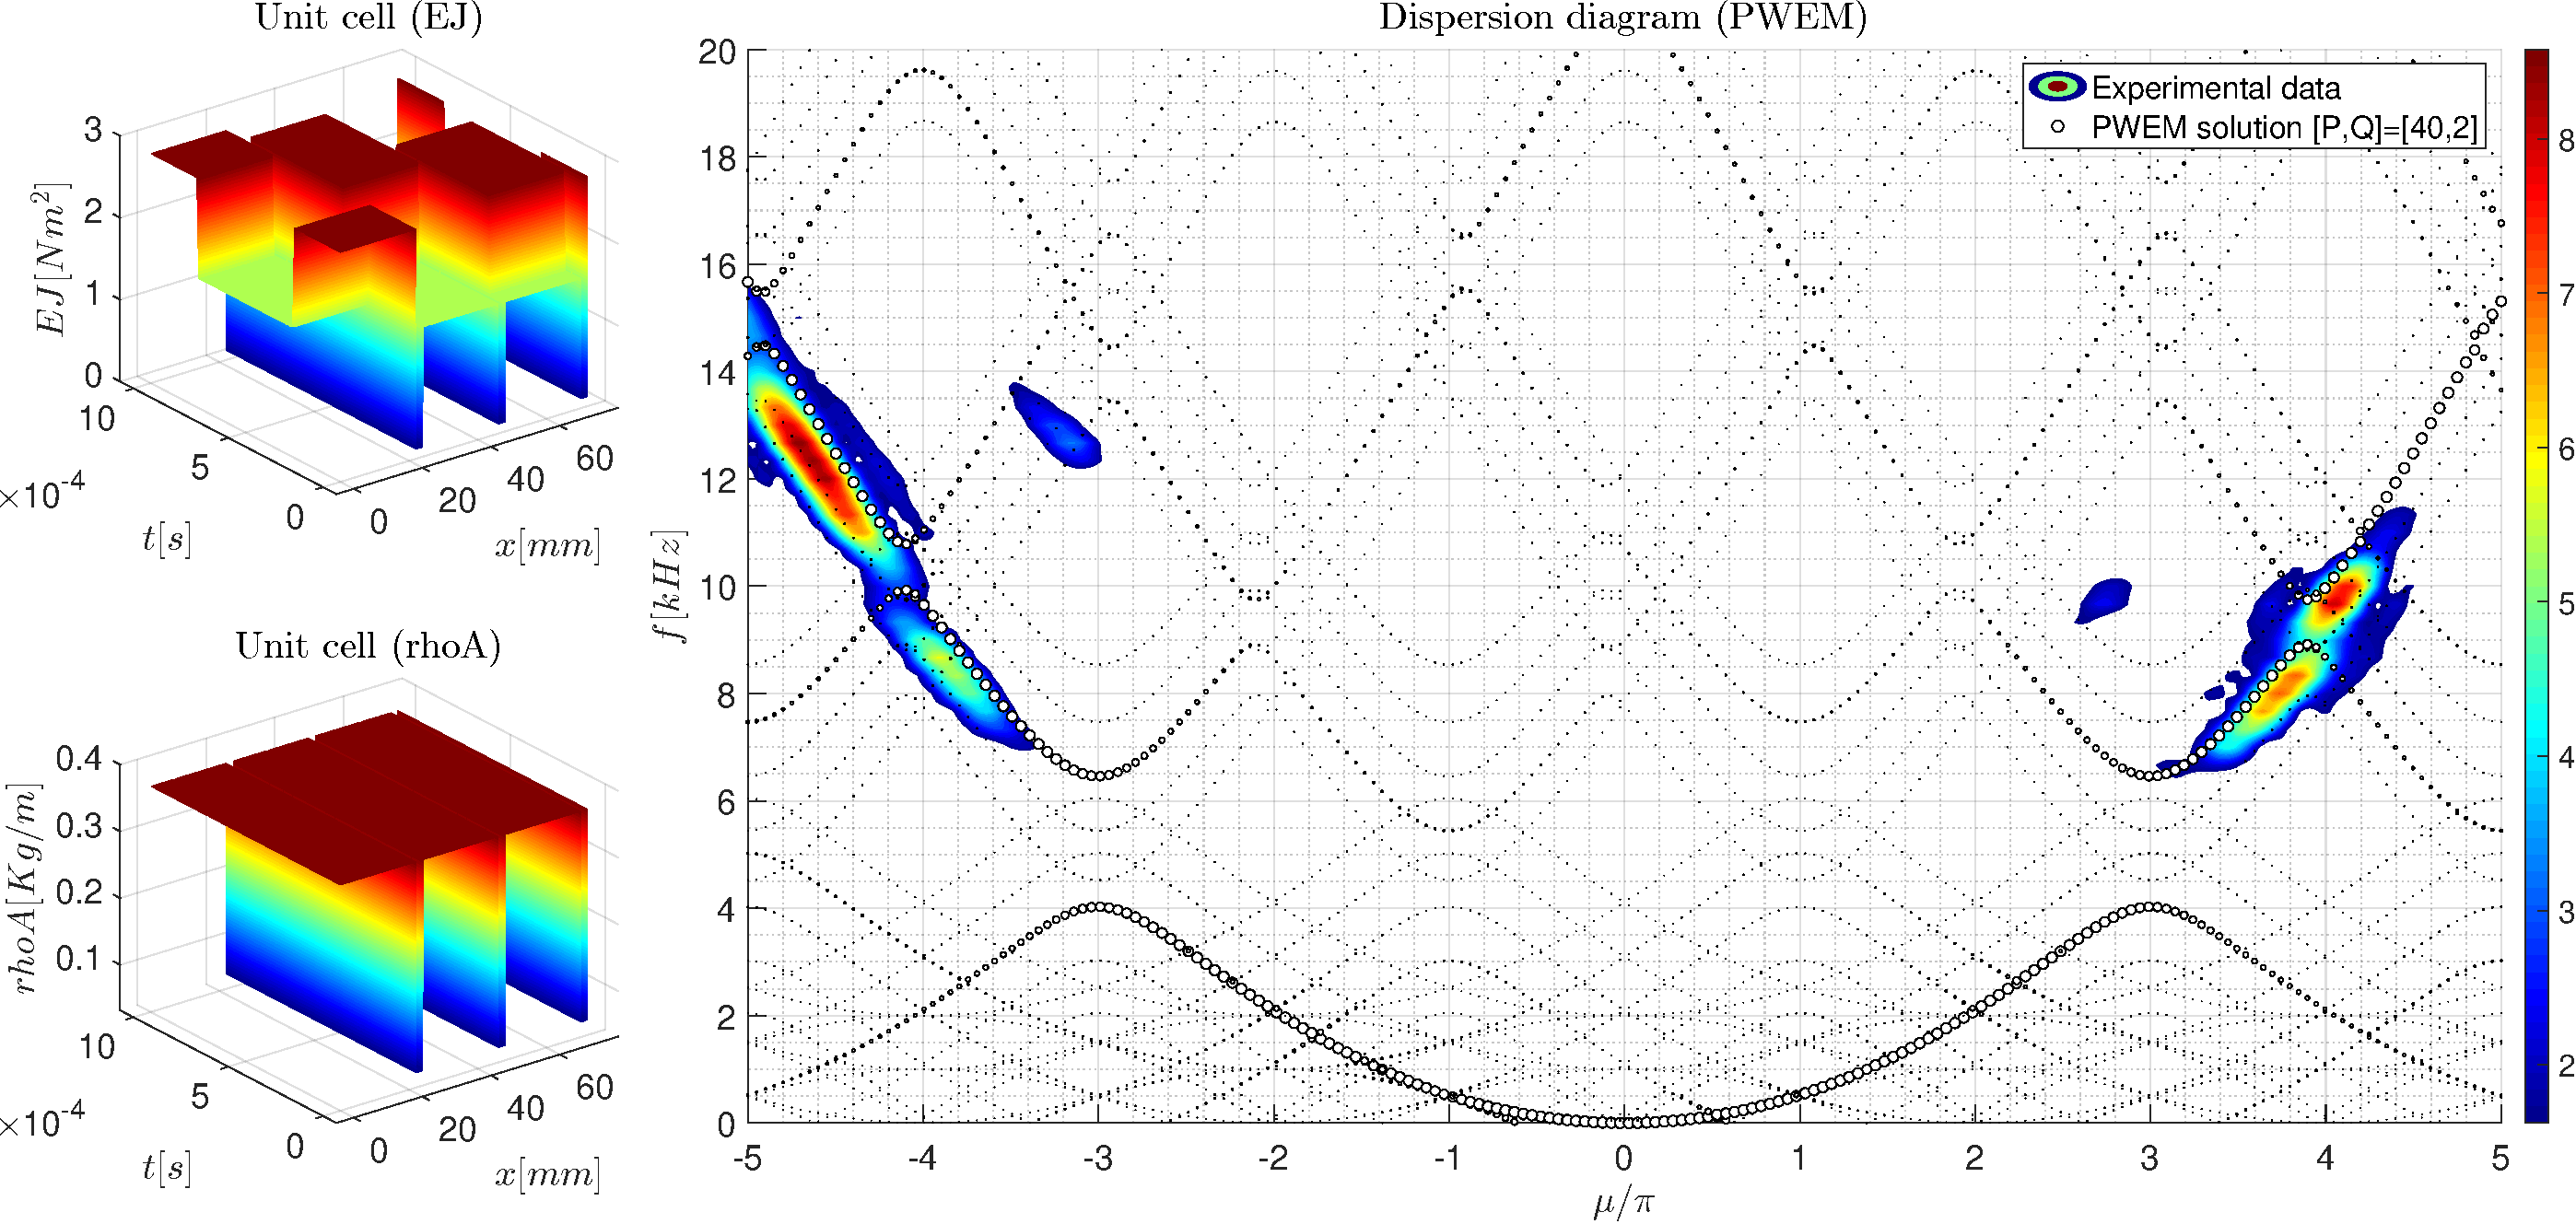
\includegraphics[width=\textwidth]{img/MATLAB/PWEM_EXP Sinusoidal (discrete) @1kHz.pdf}
    \caption{Dispersion diagram for the case of modulation frequency $f_m = \pm 1 kHz$.}
    \label{fig:PWEM_EXP_Sinusoidal_(discrete)_@1kHz}
\end{figure}

Similarly to the case of space modulation, the dispersion diagram coming from the PWEM is compared with the experimental data.
Again, except for the slight discrepancy given by the low number of harmonics considered in the PWEM, the agreement is sufficient to validate the model.

Analyzing the dispersion diagram, it's possible to observe how the first band-gap is associated with spatial modulation, while at higher frequencies nonreciprocal band-gaps associated with the time modulation appear.
In particular, it's possible to observe that at around $8.5kHz$, the first directional band-gap appears.
For the frequency range $8.5kHz < f < 9.5kHz$, we observe a band-gap for positive wavenumbers, being instead transparent in the negative wavenumber range.
On the other hand, for the frequency range $9.5kHz < f < 10.5kHz$, the band-gap is transparent for positive wavenumbers and opaque for negative wavenumbers.



\paragraph{Modulation $f_m = \pm 2 kHz$}

Similar considerations as before can be made for the case of modulation frequency $f_m = \pm 2 kHz$.

Figure \ref{fig:PWEM_EXP_Sinusoidal_(discrete)_@2kHz} shows the dispersion diagram for the case of modulation frequency $f_m = \pm 2 kHz$.

\begin{figure}[H]
    \centering
    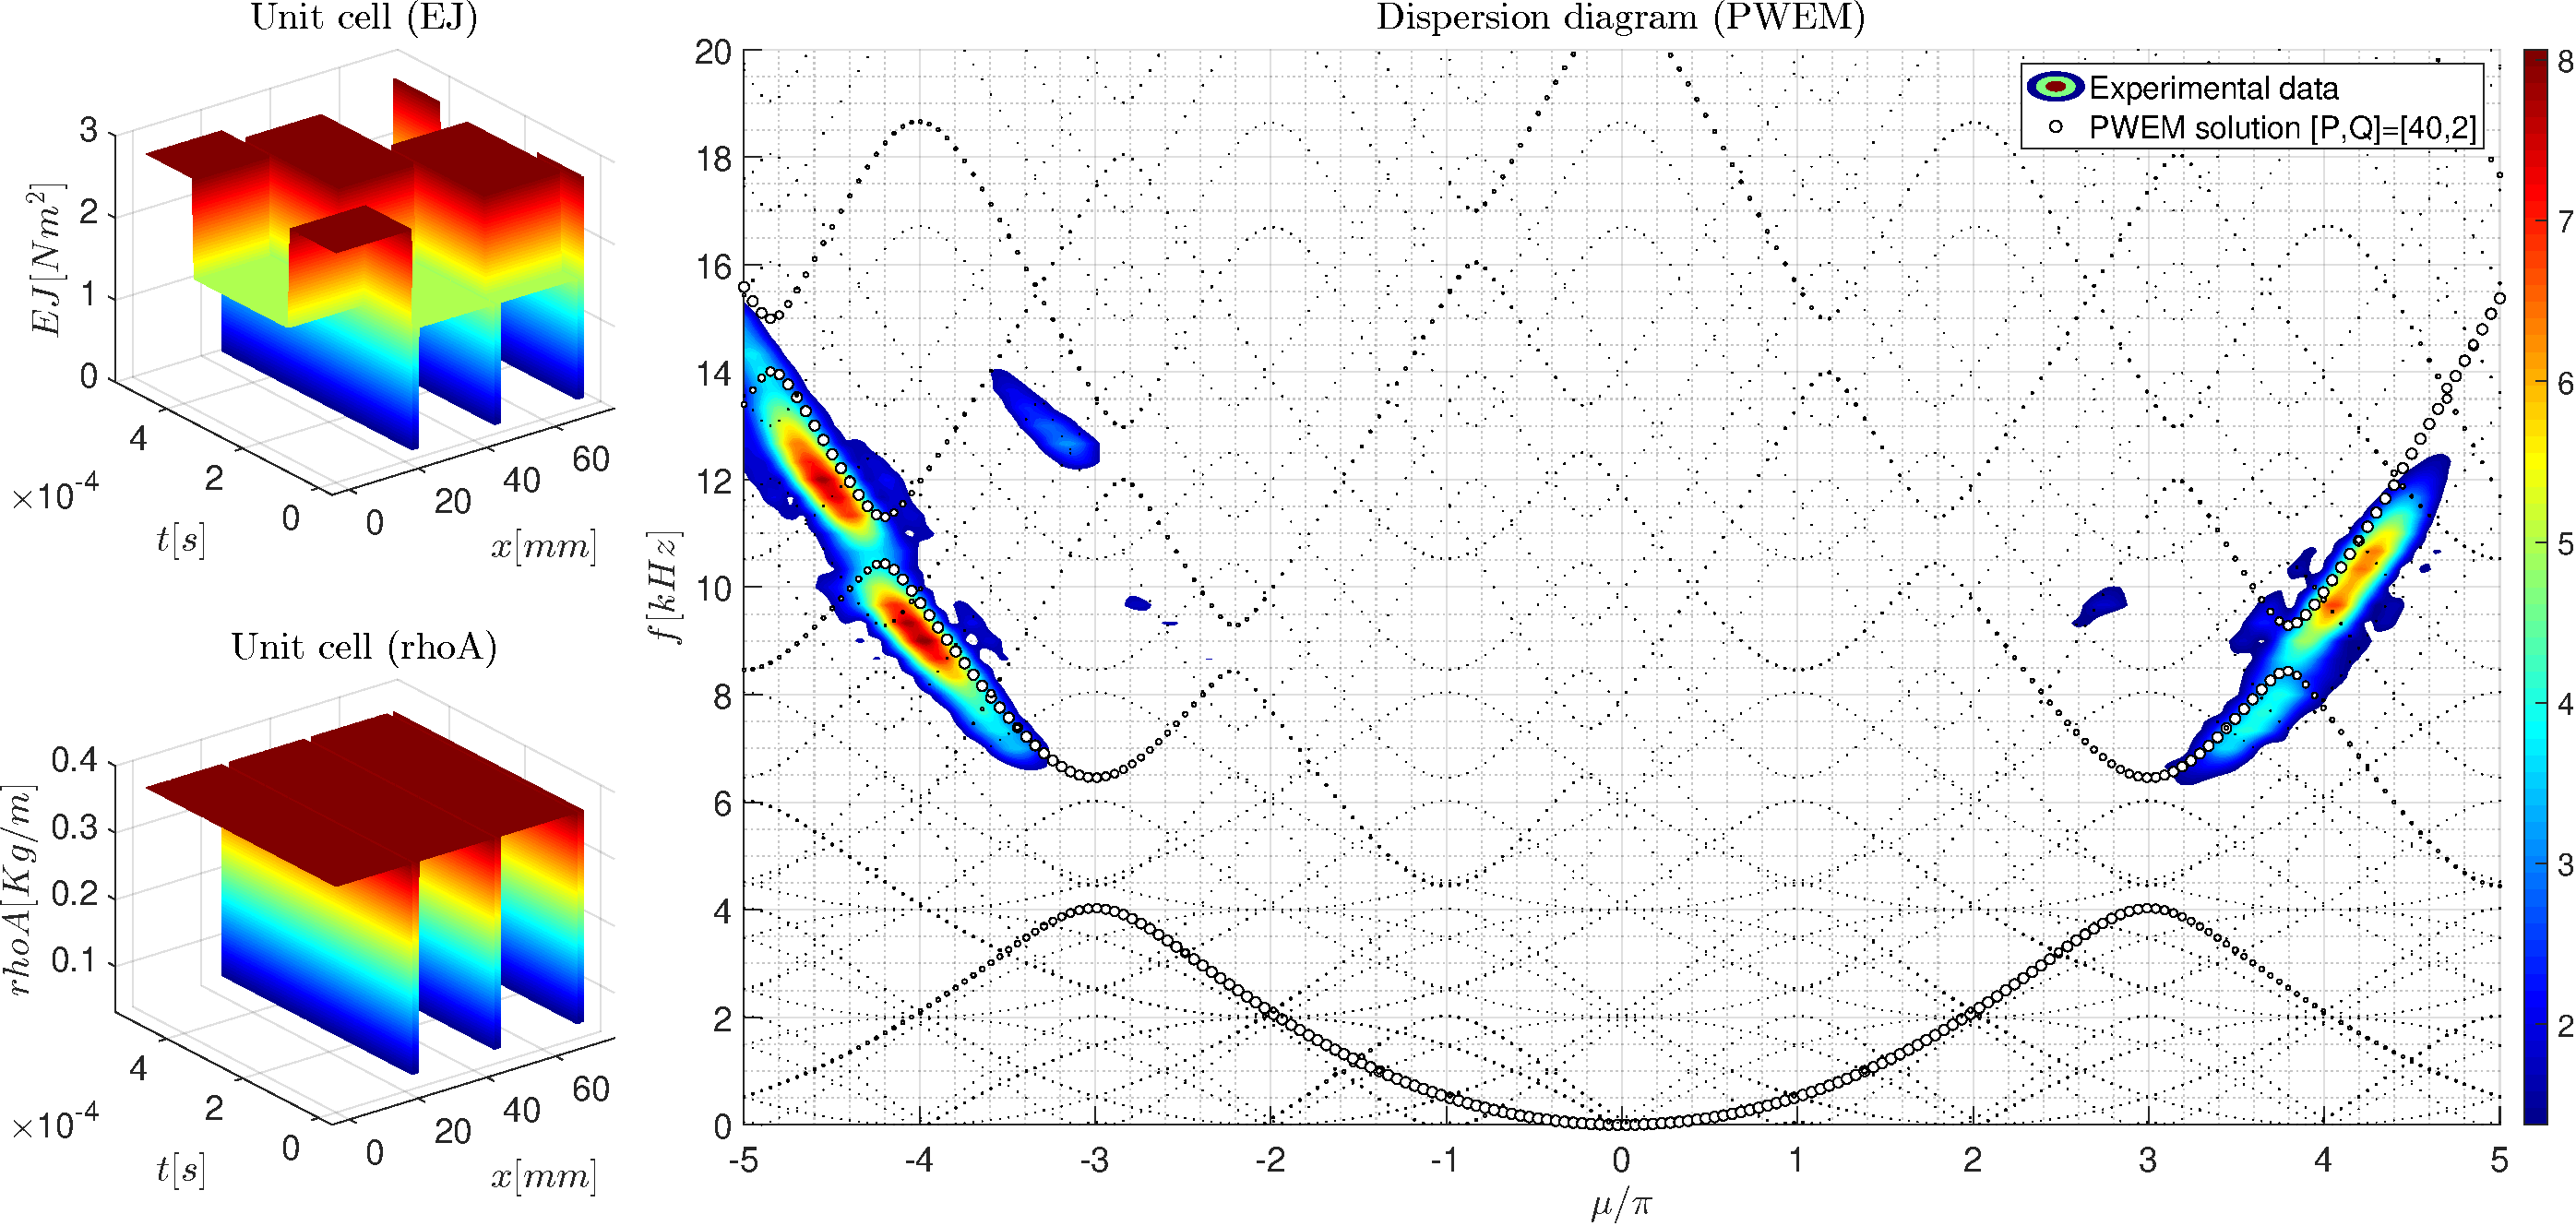
\includegraphics[width=\textwidth]{img/MATLAB/PWEM_EXP Sinusoidal (discrete) @2kHz.pdf}
    \caption{Dispersion diagram for the case of modulation frequency $f_m = \pm 2 kHz$.}
    \label{fig:PWEM_EXP_Sinusoidal_(discrete)_@2kHz}
\end{figure}

Similarly to the previous case, the dispersion diagram coming from the PWEM is compared with the experimental data.

Intuitively, the phenomenon associated with the nonreciprocal behavior is now more pronounced, as the modulation frequency is doubled.
The asymmetrical shift of the already previously analyzed directional band-gaps is even more evident.
A positive and negative shift of almost $0.5kHz$ are observed for the negative and positive wavenumbers bang-gaps, respectively.

Notice that the global band-gap at lower frequencies ($4 < f < 6.5 kHz$) is still present and hasn't been affected by the time modulation.
It's now clear that this band-gap is associated with the spatial modulation only.



\paragraph{Modulation $f_m = \pm 3 kHz$}

Figure \ref{fig:PWEM_EXP_Sinusoidal_(discrete)_@3kHz} shows the dispersion diagram for the case of modulation frequency $f_m = \pm 3 kHz$.

\begin{figure}[H]
    \centering
    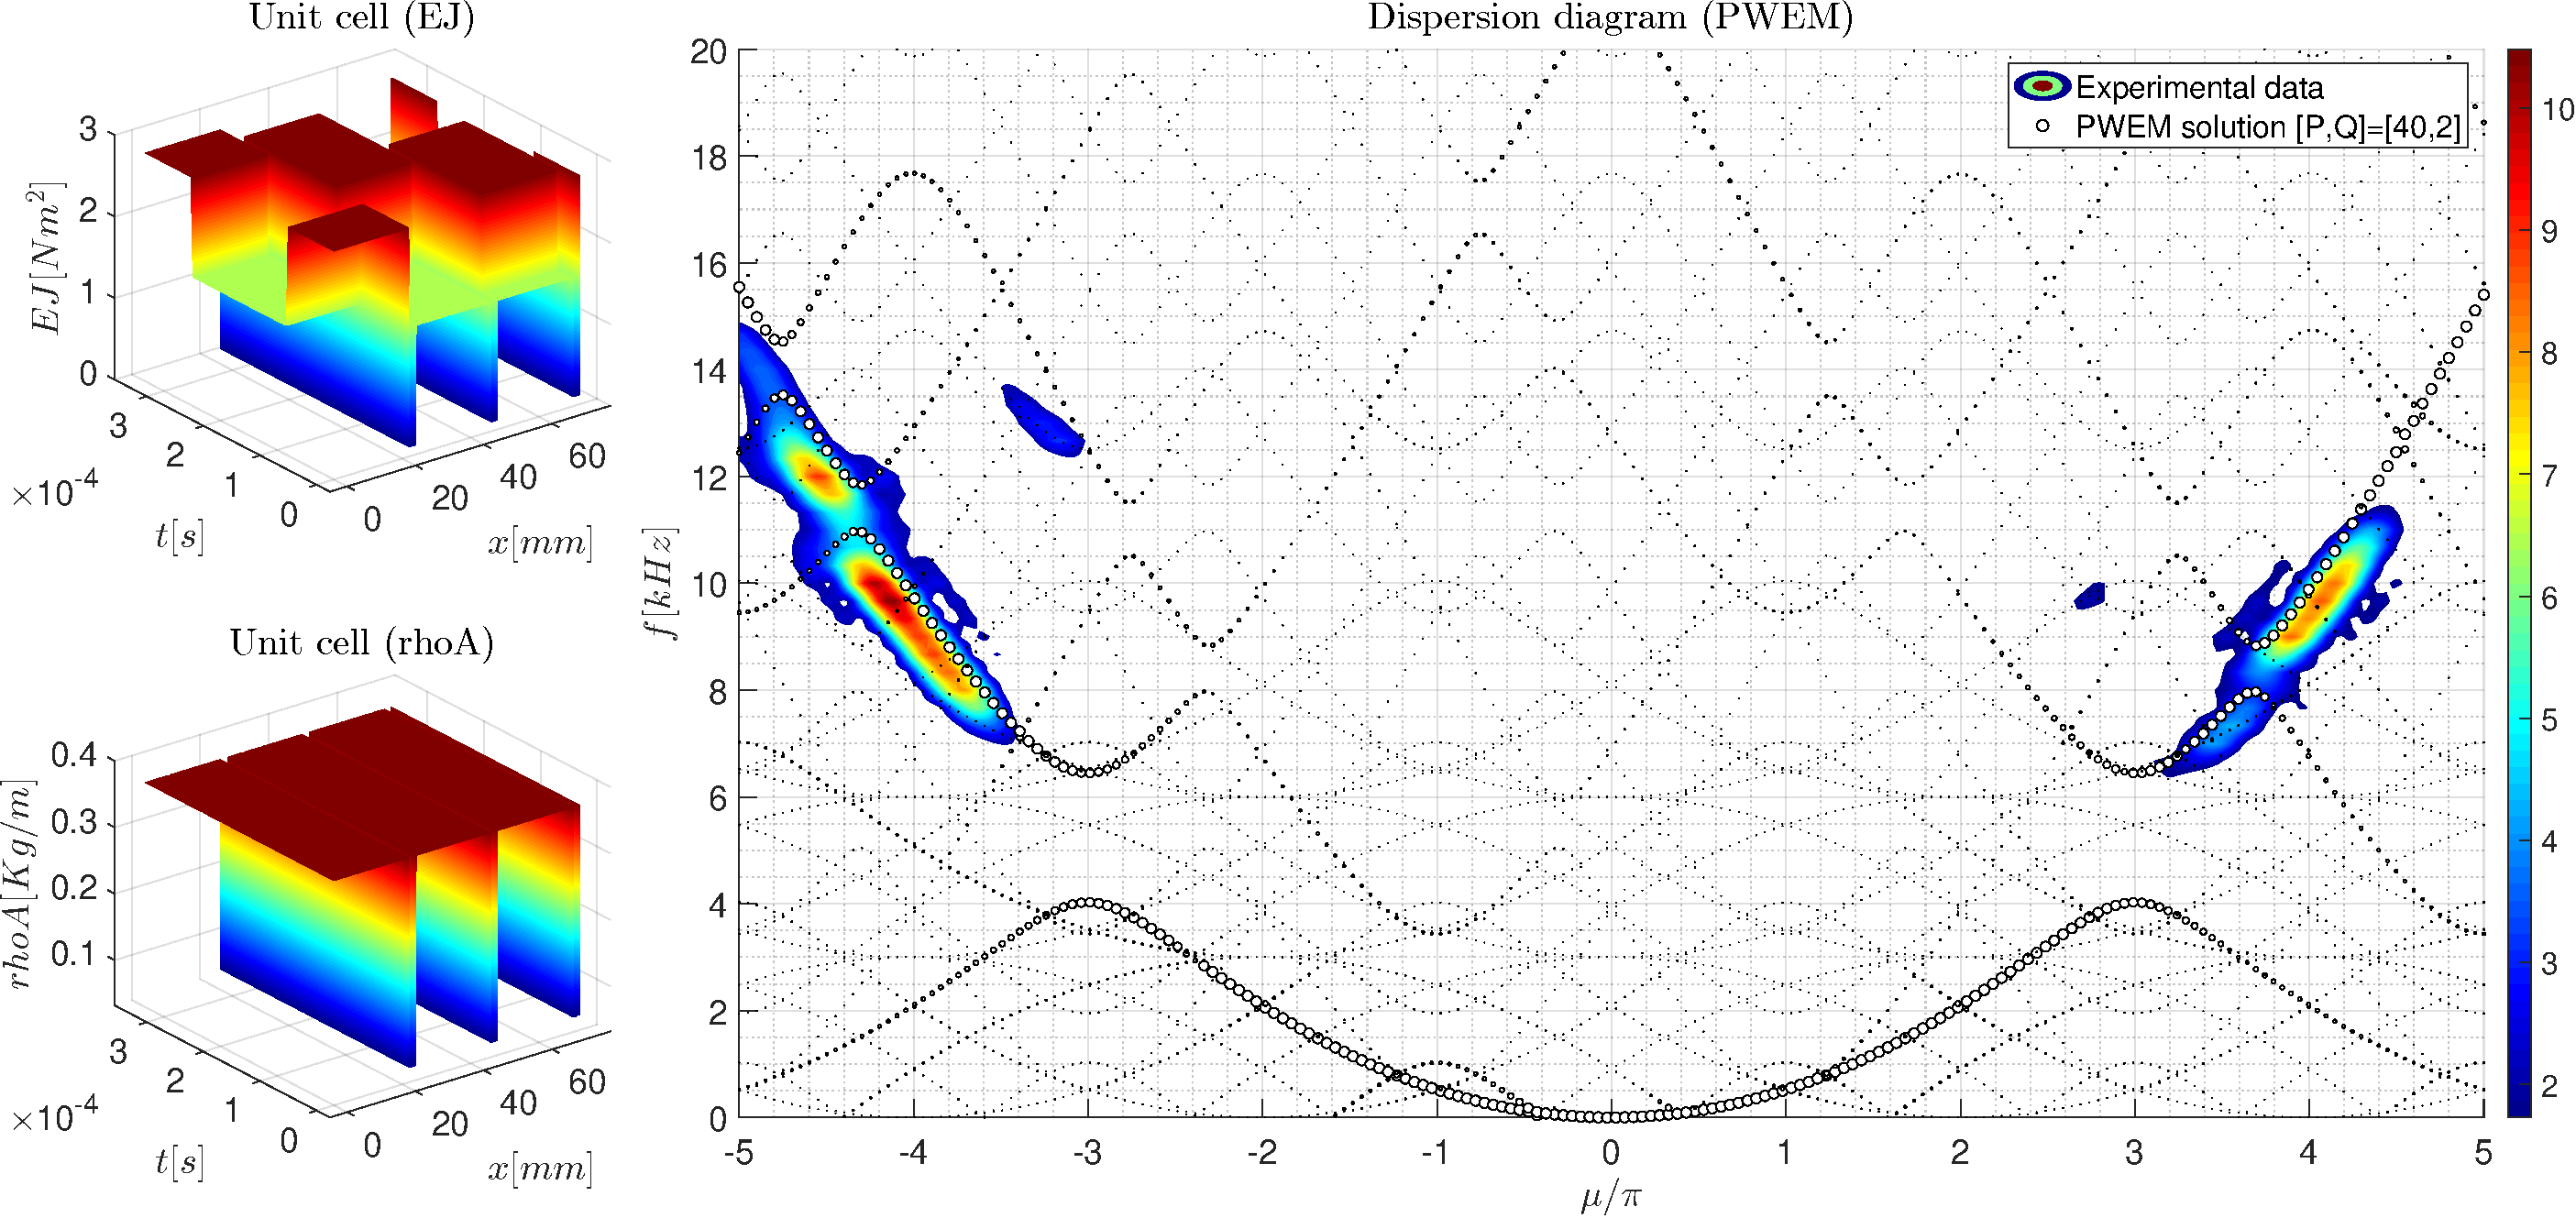
\includegraphics[width=\textwidth]{img/MATLAB/PWEM_EXP Sinusoidal (discrete) @3kHz.pdf}
    \caption{Dispersion diagram for the case of modulation frequency $f_m = \pm 3 kHz$.}
    \label{fig:PWEM_EXP_Sinusoidal_(discrete)_@3kHz}
\end{figure}

Same considerations as before can be made for the case of modulation frequency $f_m = \pm 3 kHz$.
As the modulation frequency increases, also the nonreciprocal behavior becomes more pronounced.



